% 第8章第5节：常微分方程的数值求解（显式Euler与Runge--Kutta；隐式方法与刚性；误差与步长选择）。

\section{常微分方程的数值求解}
\label{sec:ode-numerics}

大多数非线性方程没有闭式解，只能在计算机上一步一步推进。本节固定一个初值问题~\eqref{eq:ode-ivp}与有限时域$[t_0,t_0+T]$，取网格$t_n=t_0+nh$，$n=0,1,\ldots,N$，$Nh=T$，用数值状态$\widehat{\bm x}_n$近似$\bm x(t_n)$。一步数值方法是一个可计算的映射$\widehat{\bm x}_{n+1}=\bm\Psi_h(t_n,\widehat{\bm x}_n)$，它近似精确的演化映射$\bm\varphi_{t_{n+1},t_n}$。我们先构造这类映射，再看刚性怎样改变方法的选择，最后分析误差怎样从每一步累积到终点，以及怎样自动选择步长。

\subsection{显式Euler与Runge--Kutta方法}
\label{sec:ode-euler-rk}

\paragraph{冻结斜率：显式Euler}
最简单的做法是在每一小步内把斜率冻结为起点的值，沿这个方向走$h$时间，再在新位置重新读取斜率：
\begin{equation}
  \widehat{\bm x}_{n+1}=\widehat{\bm x}_n+h\,\bm g(t_n,\widehat{\bm x}_n).
  \label{eq:ode-forward-euler}
\end{equation}
这就是\term{显式Euler法}（explicit Euler method）。在斜率场图上，它相当于沿着当前箭头画一段长为$h$的直线。每步只需调用一次向量场。若向量场在一步之内变化，沿冻结方向走出的直线就会偏离真实的曲线。

衡量偏离的标准是：从精确状态出发走一步，与精确解相差多少。

\begin{definition}[局部截断误差与阶]
  \label{def:ode-local-truncation-error}
  设$\bm x$是精确解。一步方法在$t_n$处的\term{局部截断误差}为
  \[
    \bm\tau_{n+1}=\bm x(t_{n+1})-\bm\Psi_h\bigl(t_n,\bm x(t_n)\bigr).
  \]
  若存在与$n,h$无关的常数$C$，使$\|\bm\tau_{n+1}\|_2\leq Ch^{p+1}$对一切$n$与足够小的$h$成立，称方法的阶为$p$，也称其\term{收敛阶}为$p$。
\end{definition}

局部误差是$h^{p+1}$而阶数记为$p$，是因为走完固定时域需要$N=T/h$步，每步$O(h^{p+1})$的误差累计起来大约是$O(h^p)$；第~\ref{sec:ode-error-step}小节在稳定性条件下证明这一点。对显式Euler，Taylor展开给出$\bm x(t_{n+1})=\bm x(t_n)+h\dot{\bm x}(t_n)+\tfrac{h^2}2\ddot{\bm x}(\xi)$（逐分量取中间点），而$\dot{\bm x}(t_n)=\bm g(t_n,\bm x(t_n))$，所以$\bm\tau_{n+1}=O(h^2)$，阶为$1$。

\paragraph{在一步之内多看几次斜率}
要提高阶数，可以在一步之内多读几次斜率，再把它们组合起来。设$\bm g$足够光滑，沿解有$\ddot{\bm x}=\partial_t\bm g+\partial_{\bm x}\bm g\,\bm g$，于是
\[
  \bm x(t+h)=\bm x+h\bm g+\frac{h^2}2\bigl(\partial_t\bm g+\partial_{\bm x}\bm g\,\bm g\bigr)+O(h^3),
\]
右端各量在$(t,\bm x(t))$处取值。Euler法只匹配了前两项。若先用Euler走半步到中点，再在中点读取斜率，
\[
  \bm k_1=\bm g(t,\bm x),\qquad\bm k_2=\bm g\Bigl(t+\frac h2,\bm x+\frac h2\bm k_1\Bigr)=\bm g+\frac h2\bigl(\partial_t\bm g+\partial_{\bm x}\bm g\,\bm g\bigr)+O(h^2),
\]
那么$\bm x+h\bm k_2$恰好匹配到$h^2$项，局部误差为$O(h^3)$。这就是二阶的中点Runge--Kutta法（下文简称RK2）：
\begin{equation}
  \bm k_1=\bm g(t_n,\widehat{\bm x}_n),\quad
  \bm k_2=\bm g\Bigl(t_n+\frac h2,\widehat{\bm x}_n+\frac h2\bm k_1\Bigr),\quad
  \widehat{\bm x}_{n+1}=\widehat{\bm x}_n+h\bm k_2.
  \label{eq:ode-rk2}
\end{equation}
直观地说，起点的斜率只代表这一步开头的方向，中点的斜率更能代表整一步的平均方向。

沿同样的思路，用四次斜率评估、精心选取的组合系数，可以匹配到$h^4$项，得到经典的四阶Runge--Kutta法（RK4）：
\begin{equation}
  \begin{aligned}
    \bm k_1&=\bm g(t_n,\widehat{\bm x}_n),&
    \bm k_2&=\bm g\Bigl(t_n+\frac h2,\widehat{\bm x}_n+\frac h2\bm k_1\Bigr),\\
    \bm k_3&=\bm g\Bigl(t_n+\frac h2,\widehat{\bm x}_n+\frac h2\bm k_2\Bigr),&
    \bm k_4&=\bm g(t_n+h,\widehat{\bm x}_n+h\bm k_3),\\
    \widehat{\bm x}_{n+1}&=\widehat{\bm x}_n+\frac h6\bigl(\bm k_1+2\bm k_2+2\bm k_3+\bm k_4\bigr).
  \end{aligned}
  \label{eq:ode-rk4}
\end{equation}
若$\bm g$不依赖状态，RK4退化为对$\int_{t_n}^{t_{n+1}}\bm g(s)\,\mathrm ds$的Simpson求积，权重$1,4,1$中的中点权重被分给了$\bm k_2,\bm k_3$。一般地，$s$级显式\term{Runge--Kutta方法}写成
\[
  \bm k_i=\bm g\Bigl(t_n+c_ih,\widehat{\bm x}_n+h\sum_{j<i}a_{i,j}\bm k_j\Bigr),\qquad
  \widehat{\bm x}_{n+1}=\widehat{\bm x}_n+h\sum_{i=1}^sb_i\bm k_i,
\]
系数$a_{i,j},b_i,c_i$由Taylor展开的匹配条件决定，RK4满足四阶的全部条件\scite{math-hairer1993ode}。称$\bm k_i$为阶段变量；每步要调用$s$次向量场，RK2为$2$次，RK4为$4$次。

\paragraph{误差、阶数与计算量}
用一个有解析解的方程检验这些说法。取$\dot x=x\cos t$，$x(0)=1$，分离变量得$x(t)=e^{\sin t}$，终点$x(5)=e^{\sin5}\approx0.3833$。图~\ref{fig:ode-convergence-orders}(a)画出三种方法在$t=5$处的误差随步长的变化。在对数坐标下三条线近似是直线，斜率分别接近$1$、$2$、$4$：步长减半时，Euler的误差减半，RK2的误差变为四分之一，RK4的误差变为约十六分之一（例如$h=0.0098$与$0.0049$时，RK4的误差从$1.42\times10^{-11}$降到$8.9\times10^{-13}$）。

\begin{figure*}[htbp]
  \centering
  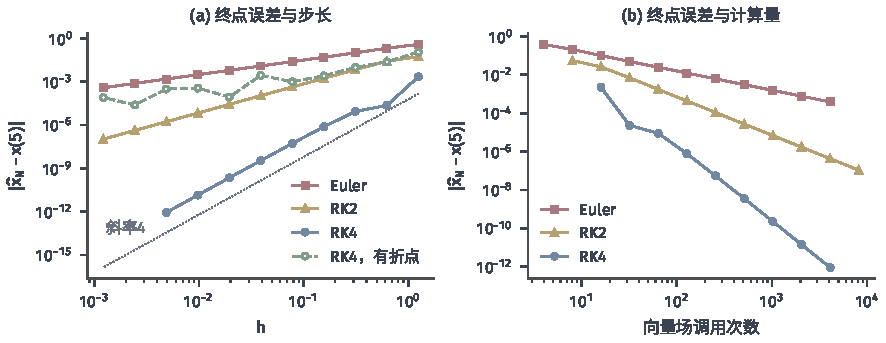
\includegraphics[width=150mm]{figures/03-optimization-evolution-and-signals/02-processes-and-trajectory-evolution/matplotlib/ode-convergence-orders/figure.pdf}
  \caption{终点误差、步长与计算量。方程$\dot x=x\cos t$，$x(0)=1$，比较$t=5$处与$e^{\sin5}$的误差，步长$h=5/2^k$（$k=2,\ldots,12$）。(a)误差对步长，点线为斜率$4$的参考线；绿色空心圆是RK4用于开关加热问题$\dot x=-0.2x+u(t)$（$u$在$t=\pi$处由$0.4$跳到$0$）的误差，跳变时刻不在网格上。(b)同样的误差对向量场调用总次数，Euler、RK2、RK4每步分别调用$1$、$2$、$4$次。}
  \label{fig:ode-convergence-orders}
\end{figure*}

比较效率时，应在同一终止时间、同一误差标准下比较总计算量，而不是比较每步的精度。图~\ref{fig:ode-convergence-orders}(b)把横轴换成向量场调用的总次数。要把误差压到约$10^{-6}$，RK4只需$32$步，即$128$次调用；RK2约需$1333$步，即约$2700$次调用；Euler则需要约$160$万步。高阶方法每步更贵，但能用大得多的步长，在光滑问题上总量反而小得多。

高阶的收益以足够的光滑性为前提。四阶的局部误差估计用到了解的五阶导数；若向量场在时间上有跳变，例如暖气在$t=\pi$时关闭而这个时刻落在某一步内部，RK4的四次斜率读数无法反映跳变发生在步内何处，那一步的局部误差只有$O(h)$量级，仅这一步就使整体误差降为一阶。图~\ref{fig:ode-convergence-orders}(a)中的绿色空心圆正是如此：误差随步长大致按一阶下降，并且随$\pi$在步内的位置而起伏。实际计算中应把已知的跳变时刻放在网格点上，在两侧分段积分。

\subsection{隐式方法与刚性问题}
\label{sec:ode-stiff}

\paragraph{快慢两种尺度}
考虑一个温度传感器：它的读数$x$以很快的速率$k=50$追随环境温度$\cos t$，
\begin{equation}
  \dot x=-k\bigl(x-\cos t\bigr),\qquad x(0)=0,\qquad k=50.
  \label{eq:ode-stiff-example}
\end{equation}
常数变易公式给出精确解$x(t)=\frac{2500\cos t+50\sin t}{2501}-\frac{2500}{2501}e^{-50t}$。最初约$0.1$个时间单位内，$e^{-50t}$项迅速消失；此后解几乎就是缓慢变化的$\cos t$。要准确描绘这条光滑曲线，步长取$0.1$到$0.2$就足够了。

显式Euler却做不到。偏差$e=x-x_{\mathrm{slow}}$近似满足$\dot e=-50e$，Euler把它每步乘以$1-50h$。$h=0.038$时因子为$-0.9$，偏差每步变号并缓慢衰减；$h=0.042$时因子为$-1.1$，偏差每步变号并放大，到$t=3$时数值解已达到约$868$。图~\ref{fig:ode-stiff}(a)画出这两种情形。为了不发散，步长必须小于$2/50=0.04$，这个限制来自早已衰减殆尽的快速分量，而不是来自我们真正想描绘的慢变化。这种“稳定性而非精度限制了显式方法的步长”的现象称为\term{刚性}（stiffness）。

\begin{figure*}[htbp]
  \centering
  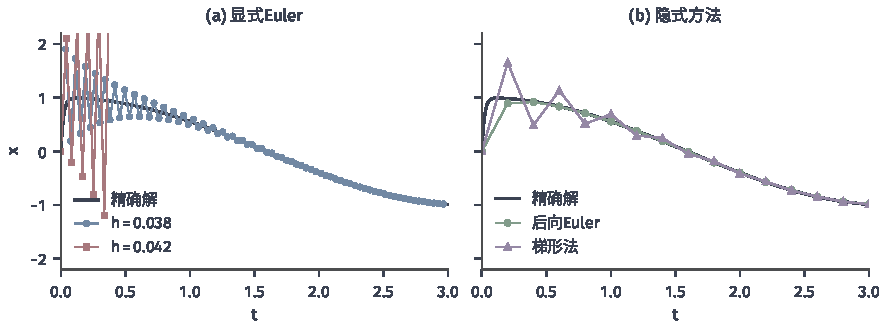
\includegraphics[width=150mm]{figures/03-optimization-evolution-and-signals/02-processes-and-trajectory-evolution/matplotlib/ode-stiff/figure.pdf}
  \caption{刚性方程$\dot x=-50(x-\cos t)$，$x(0)=0$。黑线为精确解。(a)显式Euler：$h=0.038$（蓝）时放大因子为$-0.9$，数值解振荡着缓慢靠近精确解；$h=0.042$（红）时因子为$-1.1$，数值解迅速发散（只画到超出$|x|>3$为止）。(b)步长$h=0.2$的后向Euler（绿）与梯形法（紫）：二者都不发散；后向Euler的放大因子为$1/11\approx0.091$，误差只在开头的快速过渡中可见；梯形法的放大因子为$-2/3$，开头的偏差以交替变号的方式缓慢消退。}
  \label{fig:ode-stiff}
\end{figure*}

\paragraph{线性测试方程与绝对稳定域}
为了把这个现象从具体方程中抽出来，把每个方法用于标量测试方程$\dot x=\lambda x$，$\lambda\in\mathbb C$。线性方程的一步数值映射总是乘以一个只依赖$z=h\lambda$的因子：$\widehat x_{n+1}=R(z)\widehat x_n$。显式Euler的$R(z)=1+z$；RK2与RK4的$R(z)$是$e^z$的Taylor多项式，分别截断到二次与四次：
\[
  R_{\mathrm{RK2}}(z)=1+z+\frac{z^2}2,\qquad R_{\mathrm{RK4}}(z)=1+z+\frac{z^2}2+\frac{z^3}6+\frac{z^4}{24}.
\]

\begin{definition}[绝对稳定域]
  \label{def:ode-absolute-stability}
  一步方法用于测试方程$\dot x=\lambda x$时给出$\widehat x_{n+1}=R(h\lambda)\widehat x_n$。集合$\mathcal S=\{z\in\mathbb C:|R(z)|\leq1\}$称为方法的\term{绝对稳定域}。若$\mathcal S$包含整个闭左半平面$\{\operatorname{Re}z\leq0\}$，称方法\term{A稳定}。
\end{definition}

对线性系统$\dot{\bm x}=\bm A\bm x$，若$\bm A$可对角化，方法在特征坐标下对每个特征值分别作用，数值解不增长的条件是每个$h\lambda_i$都落在$\mathcal S$中。这里要分清两种稳定性：方程的稳定性问的是$\operatorname{Re}\lambda<0$，即精确解是否衰减；方法的稳定性问的是$h\lambda\in\mathcal S$，即数值解是否衰减。前者是方程的性质，后者还依赖步长和方法。

图~\ref{fig:ode-stability-regions}(a)画出三个显式方法的稳定域。Euler的稳定域是以$-1$为心的单位圆盘；RK2稍大，在实轴上同样止于$-2$；RK4更大，在实轴上延伸到约$-2.785$，并且包含虚轴上的一段$|y|\leq2\sqrt2$。刚性例子中$\lambda=-50$，三者的步长上限依次约为$0.04$、$0.04$、$0.056$。显式Runge--Kutta方法的$R$是多项式，$|z|\to\infty$时$|R(z)|\to\infty$，所以稳定域总是有界的，不可能A稳定。提高阶数可以把稳定域扩大一些，却解除不了刚性带来的限制。

\begin{figure*}[htbp]
  \centering
  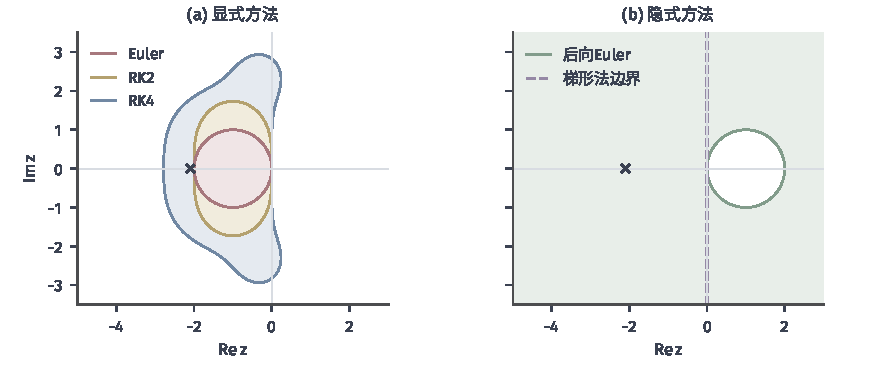
\includegraphics[width=150mm]{figures/03-optimization-evolution-and-signals/02-processes-and-trajectory-evolution/matplotlib/ode-stability-regions/figure.pdf}
  \caption{线性测试方程$\dot x=\lambda x$下的绝对稳定域$\{z=h\lambda:|R(z)|\leq1\}$。(a)显式方法：Euler（红，圆盘）、RK2（黄）、RK4（蓝）；三者在负实轴上分别止于$-2$、$-2$、约$-2.785$。(b)隐式方法：后向Euler的稳定域是以$1$为心的单位圆盘之外的全部区域（绿色填充），梯形法的稳定域恰为闭左半平面（紫色虚线为其边界）。两图中的叉号标出$z=-2.1$。}
  \label{fig:ode-stability-regions}
\end{figure*}

\paragraph{隐式方法}
显式方法只用起点的信息。若改用终点的斜率，
\begin{equation}
  \widehat{\bm x}_{n+1}=\widehat{\bm x}_n+h\,\bm g(t_{n+1},\widehat{\bm x}_{n+1}),
  \label{eq:ode-backward-euler}
\end{equation}
得到\term{后向Euler法}（backward Euler method）。未知的$\widehat{\bm x}_{n+1}$同时出现在两边，每一步都要解一个方程，所以称为隐式方法。用于测试方程，$\widehat x_{n+1}=\widehat x_n+z\widehat x_{n+1}$，即$R(z)=1/(1-z)$；当$\operatorname{Re}z\leq0$时$|1-z|\geq1$，所以后向Euler是A稳定的。它的稳定域甚至包含右半平面的大部分，只排除以$1$为心的单位圆盘。

把起点与终点的斜率平均，得到\term{梯形法}：
\begin{equation}
  \widehat{\bm x}_{n+1}=\widehat{\bm x}_n+\frac h2\Bigl(\bm g(t_n,\widehat{\bm x}_n)+\bm g(t_{n+1},\widehat{\bm x}_{n+1})\Bigr),
  \label{eq:ode-trapezoid}
\end{equation}
其$R(z)=(1+z/2)/(1-z/2)$。$|R(z)|\leq1$恰好等价于$\operatorname{Re}z\leq0$，所以梯形法的稳定域就是闭左半平面：它A稳定，而且是二阶的，后向Euler只有一阶。

A稳定只保证数值解不增长，不保证快速分量被迅速抹去。当$z\to-\infty$时，后向Euler的$R(z)\to0$，快速分量一步就几乎消失；梯形法的$R(z)\to-1$，快速分量几乎不衰减，只是每步变号。对刚性例子取$h=0.2$，$z=-10$，后向Euler的因子为$1/11\approx0.091$，梯形法为$-2/3$；若$h=2$，$z=-100$，梯形法的因子为$-49/51\approx-0.961$，开头的偏差要振荡很久才消退。图~\ref{fig:ode-stiff}(b)显示了$h=0.2$时的差别：后向Euler的误差只在开头的快速过渡中出现，最大约$0.093$；梯形法第一步给出$1.650$，而精确值为$0.984$，此后的偏差交替变号、按$2/3$的比例消退。是否需要强阻尼，取决于是否关心快速过渡阶段本身。

\paragraph{隐式方程怎样求解}
线性方程$\dot{\bm x}=\bm A\bm x+\bm b(t)$的后向Euler步是线性方程组
\[
  (\bm I-h\bm A)\,\widehat{\bm x}_{n+1}=\widehat{\bm x}_n+h\,\bm b(t_{n+1}).
\]
步长固定时，系数矩阵不变，可以只做一次LU分解，以后每步只需回代。刚性例子是标量情形，直接得到$\widehat x_{n+1}=(\widehat x_n+50h\cos t_{n+1})/(1+50h)$。

非线性方程要解$\bm G(\bm y)=\bm y-\widehat{\bm x}_n-h\bm g(t_{n+1},\bm y)=\bm0$。最直接的想法是不动点迭代$\bm y\leftarrow\widehat{\bm x}_n+h\bm g(t_{n+1},\bm y)$，可它是压缩的条件恰是$hL<1$；刚性问题的$L$很大，这个条件与显式方法的步长限制一样苛刻，隐式方法的好处就丢掉了。所以通常用Newton法：从显式Euler给出的预测值出发，反复求解
\[
  \bigl(\bm I-h\,\partial_{\bm x}\bm g(t_{n+1},\bm y^{(k)})\bigr)\bm\delta=-\bm G(\bm y^{(k)}),\qquad\bm y^{(k+1)}=\bm y^{(k)}+\bm\delta.
\]
Newton法在解附近二次收敛，其条件与性质可参考第~\ref{chap:opt-smooth}章。每次迭代需要Jacobian矩阵和一次$d\times d$线性方程组的求解，稠密情形代价为$O(d^3)$；实际中常在若干步之间重用同一个Jacobian及其分解，以牺牲一些收敛速度换取更低的代价。显式方法每步只需若干次向量场调用。因此，隐式方法以更贵的单步换取大得多的稳定步长，只在刚性问题上划算。迭代在有限次后停止，留下的残差相当于每步额外加入的一个小扰动，下一小节把它与截断误差、舍入误差放在一起分析。

后向Euler和梯形法都只用当前一步的信息。线性多步方法还利用前几步的状态，例如二阶后向差分公式
\[
  \frac32\widehat{\bm x}_{n+1}-2\widehat{\bm x}_n+\frac12\widehat{\bm x}_{n-1}=h\,\bm g(t_{n+1},\widehat{\bm x}_{n+1}),
\]
每步只解一个隐式方程就达到二阶，并且A稳定；代价是需要额外的起步值，变步长也更麻烦。A稳定的线性多步方法阶数不超过二，这是多步方法的一个基本限制\scite{math-suli2003numerical}。本书不展开多步方法。

\subsection{局部误差、全局误差与步长选择}
\label{sec:ode-error-step}

\paragraph{误差扇：局部误差怎样累积}
每一步的局部误差都把数值解推到一条邻近的精确解上；此后，精确的动力学会把这条邻近解带向何方，就决定了这个局部误差在终点变成多少。图~\ref{fig:ode-error-fan}把这一过程画出来：从每个数值点出发画一条精确解，红色竖线是每一步的局部误差。

\begin{figure*}[htbp]
  \centering
  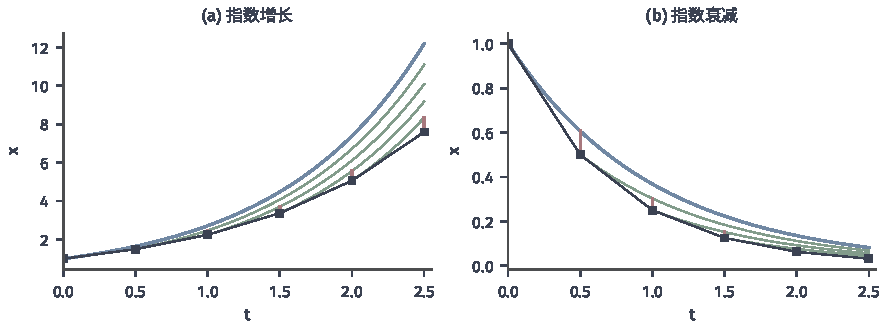
\includegraphics[width=150mm]{figures/03-optimization-evolution-and-signals/02-processes-and-trajectory-evolution/matplotlib/ode-error-fan/figure.pdf}
  \caption{局部误差的传播。显式Euler，步长$h=0.5$，$x(0)=1$，黑色方块为数值解，蓝色是精确解，绿色是从各数值点出发的精确解，红色竖线是每步的局部误差。(a)$\dot x=x$：五个局部误差约为$0.149,0.223,0.335,0.502,0.753$，被增长的流逐步放大，终点误差约为$4.59$。(b)$\dot x=-x$：局部误差约为$0.107,0.053,0.027,0.013,0.007$，被收缩的流逐步抹平，终点误差约为$0.051$。}
  \label{fig:ode-error-fan}
\end{figure*}

两种情形形成鲜明对比。在增长的方程$\dot x=x$中，绿色曲线像扇面一样张开，越早产生的局部误差被放大得越多，终点误差$4.59$远大于局部误差之和$1.96$。在衰减的方程$\dot x=-x$中，绿色曲线相互靠拢，早期的局部误差被逐渐遗忘，终点误差$0.051$小于局部误差之和$0.207$。全局误差由两个因素共同决定：每步产生多少局部误差，以及动力学把它们放大还是缩小。

\paragraph{相容性加稳定性给出收敛}
把这幅图写成不等式。记全局误差$\bm e_n=\widehat{\bm x}_n-\bm x(t_n)$，并允许每步计算带有一个额外扰动$\bm\eta_n$，它可以来自舍入误差，也可以来自隐式方程没有解准的残差：$\widehat{\bm x}_{n+1}=\bm\Psi_h(t_n,\widehat{\bm x}_n)+\bm\eta_n$。于是
\[
  \bm e_{n+1}=\underbrace{\bm\Psi_h(t_n,\widehat{\bm x}_n)-\bm\Psi_h\bigl(t_n,\bm x(t_n)\bigr)}_{\text{已有误差经一步传播}}-\underbrace{\bm\tau_{n+1}}_{\text{局部截断误差}}+\bm\eta_n.
\]
第一项需要数值映射本身不过分放大差别，第二项需要局部误差小。前者称为稳定性，后者称为\term{相容性}（consistency）。下面的离散Grönwall不等式把两者合起来。

\begin{lemma}[离散Grönwall不等式]
  \label{lem:ode-discrete-gronwall}
  设非负数列$\epsilon_n$满足$\epsilon_{n+1}\leq(1+\Lambda h)\epsilon_n+\beta$，其中$\Lambda>0$，$h,\beta\geq0$。则
  \[
    \epsilon_n\leq e^{\Lambda nh}\epsilon_0+\frac{e^{\Lambda nh}-1}{\Lambda h}\,\beta.
  \]
\end{lemma}

\begin{proof}
  归纳展开得$\epsilon_n\leq(1+\Lambda h)^n\epsilon_0+\beta\sum_{j=0}^{n-1}(1+\Lambda h)^j=(1+\Lambda h)^n\epsilon_0+\beta\frac{(1+\Lambda h)^n-1}{\Lambda h}$，再用$1+\Lambda h\leq e^{\Lambda h}$。
\end{proof}

\begin{theorem}[一步方法的有限时域收敛]
  \label{thm:ode-one-step-convergence}
  设精确解$\bm x$在$[t_0,t_0+T]$上存在，$K$是包含精确解与数值解的集合。设
  \begin{enumerate}
    \item （相容性）$\|\bm\tau_{n+1}\|_2\leq Ch^{p+1}$对一切$n$成立；
    \item （稳定性）$\|\bm\Psi_h(t,\bm y)-\bm\Psi_h(t,\bm z)\|_2\leq(1+\Lambda h)\|\bm y-\bm z\|_2$对$\bm y,\bm z\in K$成立，$\Lambda>0$；
    \item （扰动）$\|\bm\eta_n\|_2\leq\eta$对一切$n$成立。
  \end{enumerate}
  则对$nh\leq T$，
  \begin{equation}
    \|\bm e_n\|_2\leq e^{\Lambda T}\|\bm e_0\|_2+\frac{e^{\Lambda T}-1}{\Lambda}\Bigl(Ch^p+\frac\eta h\Bigr).
    \label{eq:ode-global-error}
  \end{equation}
\end{theorem}

\begin{proof}
  由误差递推式及三条假设，$\|\bm e_{n+1}\|_2\leq(1+\Lambda h)\|\bm e_n\|_2+Ch^{p+1}+\eta$。应用引理~\ref{lem:ode-discrete-gronwall}，取$\beta=Ch^{p+1}+\eta$，并用$nh\leq T$。
\end{proof}

式~\eqref{eq:ode-global-error}的三项各有含义。初值误差最多被放大$e^{\Lambda T}$倍，与连续依赖的估计一致。截断误差每步$Ch^{p+1}$，约$T/h$步累计成$O(h^p)$，这就是“局部$h^{p+1}$、全局$h^p$”的来源。每步扰动$\eta$也累计$T/h$次，变成$\eta/h$：步长越小，步数越多，舍入误差积累得越多。所以不断减小步长并不能无限提高精度，存在一个最佳步长，使$Ch^p$与$\eta/h$大致相当。双精度计算的舍入误差约为$10^{-16}$量级，对低阶方法这个下限通常远低于所需精度，对高阶方法和很严的容差则会显现。

对显式Euler，若$\bm g$在$K$上关于状态有Lipschitz常数$L$，则$\|\bm\Psi_h(t,\bm y)-\bm\Psi_h(t,\bm z)\|_2\leq(1+hL)\|\bm y-\bm z\|_2$，稳定性条件对$\Lambda=L$成立；若精确解满足$\|\ddot{\bm x}\|_2\leq M_2$，则$C=M_2/2$。代入式~\eqref{eq:ode-global-error}，从精确初值出发、无额外扰动时得到
\begin{equation}
  \|\widehat{\bm x}_n-\bm x(t_n)\|_2\leq\frac{M_2h}{2L}\bigl(e^{LT}-1\bigr).
  \label{eq:ode-euler-global-error}
\end{equation}
显式Runge--Kutta方法的阶段变量都是$\bm g$的Lipschitz函数，对$h\leq h_0$同样有某个$\Lambda$满足稳定性条件，再配合$p$阶的相容性就得到$O(h^p)$的全局误差。

\paragraph{用方向而不只是大小：单侧Lipschitz条件}
式~\eqref{eq:ode-global-error}中的$e^{\Lambda T}$用的是Lipschitz常数，与第~\ref{sec:ode-continuous-dependence}小节的连续依赖估计有同样的缺点：它只看向量场变化的大小，不看方向。对刚性例子，$L=50$，$e^{50T}$是一个天文数字，估计毫无用处，尽管精确解和后向Euler都在收缩差别。改进的办法是只看差别方向上的分量。若存在$\nu\in\mathbb R$使
\[
  \bigl\langle\bm g(t,\bm y)-\bm g(t,\bm z),\bm y-\bm z\bigr\rangle\leq\nu\|\bm y-\bm z\|_2^2
\]
对一切$\bm y,\bm z$成立，称$\bm g$满足单侧Lipschitz条件，常数$\nu$可以为负。刚性例子中$\nu=-50$，温度模型中$\nu=-\lambda$。

这个条件同时控制精确流和后向Euler。对两条精确解，$\frac{\mathrm d}{\mathrm dt}\frac12\|\bm x-\widetilde{\bm x}\|_2^2\leq\nu\|\bm x-\widetilde{\bm x}\|_2^2$，所以差别按$e^{\nu t}$变化：$\nu<0$时收缩。这正好弥补了第~\ref{sec:ode-continuous-dependence}小节中温度模型的Grönwall上界随时间增长的缺陷。对后向Euler，设两个起点$\bm a,\bm b$分别给出$\bm y,\bm z$，即$\bm y-h\bm g(\bm y)=\bm a$、$\bm z-h\bm g(\bm z)=\bm b$（省略时间变量）。两式相减后与$\bm y-\bm z$作内积，
\[
  \|\bm y-\bm z\|_2^2-h\bigl\langle\bm g(\bm y)-\bm g(\bm z),\bm y-\bm z\bigr\rangle=\langle\bm a-\bm b,\bm y-\bm z\rangle\leq\|\bm a-\bm b\|_2\|\bm y-\bm z\|_2,
\]
左端不小于$(1-h\nu)\|\bm y-\bm z\|_2^2$。所以当$h\nu<1$时，
\[
  \|\bm y-\bm z\|_2\leq\frac{\|\bm a-\bm b\|_2}{1-h\nu}.
\]
$\nu\leq0$时，后向Euler的一步映射对任何步长都不放大差别，稳定性常数与刚性强弱无关。这就是隐式方法在刚性问题上能给出有用误差界的原因。

\paragraph{嵌入式方法估计局部误差}
理论误差界中的常数通常未知，实际计算需要从计算结果本身估计误差，并据此调整步长。最常用的办法是嵌入式方法：用同一组阶段变量构造两个不同阶数的更新，二者之差估计较低阶更新的局部误差。最简单的一对是Heun--Euler对：
\[
  \begin{gathered}
  \bm k_1=\bm g(t_n,\widehat{\bm x}_n),\quad\bm k_2=\bm g(t_n+h,\widehat{\bm x}_n+h\bm k_1),\\
  \bm x^{[1]}=\widehat{\bm x}_n+h\bm k_1,\quad\bm x^{[2]}=\widehat{\bm x}_n+\frac h2(\bm k_1+\bm k_2).
  \end{gathered}
\]
$\bm x^{[1]}$是一阶的Euler步，$\bm x^{[2]}$是二阶的Heun步，二者共用两次向量场调用。由于$\bm x^{[2]}$的局部误差比$\bm x^{[1]}$高一阶，差值$\mathrm{err}=\|\bm x^{[2]}-\bm x^{[1]}\|=\frac h2\|\bm k_2-\bm k_1\|$在主项上等于$\bm x^{[1]}$的局部误差。另一种办法是步长加倍：分别用一步$h$和两步$h/2$推进，比较两个结果。

有了误差估计，步长控制按如下规则进行。给定容差$\mathrm{tol}$：若$\mathrm{err}\leq\mathrm{tol}$，接受这一步，并通常用较高阶的$\bm x^{[2]}$继续（称为局部外推）；否则拒绝，用更小的步长重算这一步。无论接受与否，下一个步长都取
\[
  h_{\mathrm{new}}=h\cdot\min\Bigl\{f_{\max},\ \max\Bigl\{f_{\min},\ 0.9\Bigl(\frac{\mathrm{tol}}{\mathrm{err}}\Bigr)^{1/(q+1)}\Bigr\}\Bigr\},
\]
其中$q$是被估计误差的那个更新的阶（Heun--Euler对中$q=1$）。理由是局部误差约为$Ch^{q+1}$，要让它恰好等于$\mathrm{tol}$，步长应乘以$(\mathrm{tol}/\mathrm{err})^{1/(q+1)}$；因子$0.9$留出安全余量，$f_{\min},f_{\max}$（例如$0.2$与$2$）防止步长剧烈跳动。

\begin{figure}[htbp]
  \centering
  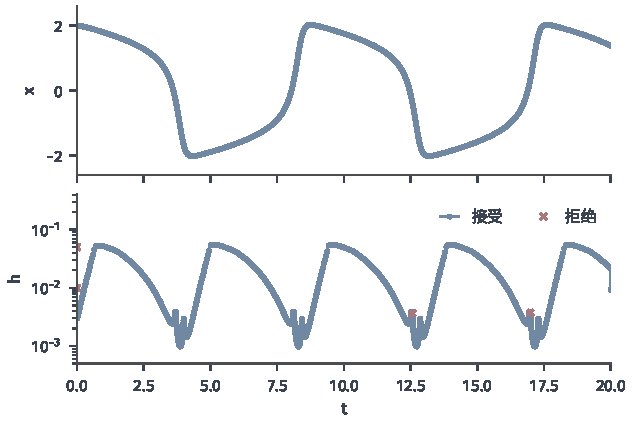
\includegraphics[width=107mm]{figures/03-optimization-evolution-and-signals/02-processes-and-trajectory-evolution/matplotlib/ode-adaptive-step/figure.pdf}
  \caption{自适应步长。van der Pol方程$\dot x=y$，$\dot y=3(1-x^2)y-x$，从$(2,0)$出发计算到$t=20$，使用Heun--Euler对，最大范数容差$10^{-4}$，$f_{\min}=0.2$，$f_{\max}=2$。上图：黑线为参考解的$x$分量，蓝点为接受的数值点。下图：接受的步长（蓝，对数纵轴）与被拒绝的尝试步长（红叉）。}
  \label{fig:ode-adaptive-step}
\end{figure}

图~\ref{fig:ode-adaptive-step}把这个规则用于$\mu=3$的van der Pol方程。解在缓慢漂移与急剧翻转之间交替；步长随之在约$0.056$与$0.00098$之间变化，翻转时自动缩小，漂移时自动放大。全程接受$3221$步、拒绝$4$次，共调用向量场$6450$次；若始终使用最小步长，则需要约$2.0$万步。$t=20$处的实际误差约为$9\times10^{-6}$。

\paragraph{局部误差控制的边界}
自适应方法控制的是每步的局部误差，不是终点的全局误差。误差扇说明，同样的局部误差在增长的动力学下会被放大$e^{\Lambda T}$倍；容差满足了，终点误差仍可能很大，长时间计算或对初值敏感的系统尤其如此。局部误差控制也不保证守恒量或几何结构：对无阻尼的振动系统，每步都合格的误差仍可能沿一个方向持续积累，使能量缓慢漂移，下一节专门处理这个问题。若把显式自适应方法用于刚性问题，步长控制器会发现：步长稍大，快速分量的不稳定就使误差估计变大，于是步长被一再压到稳定极限附近，计算量猛增。这是刚性的一个实用信号，应改用隐式方法。
